% !TeX root = ../dd.tex

\section{Architectural Design}

\subsection{Overview}
% High-level component and their interaction
To ensure high maintainability, scalability and security, the service is structured according to the well-established three-tier architecture.
Figure \ref{fig:overview-architecture} shows how the tiers are divided, and what are the relations between key components of the system.

\begin{figure}[H]
    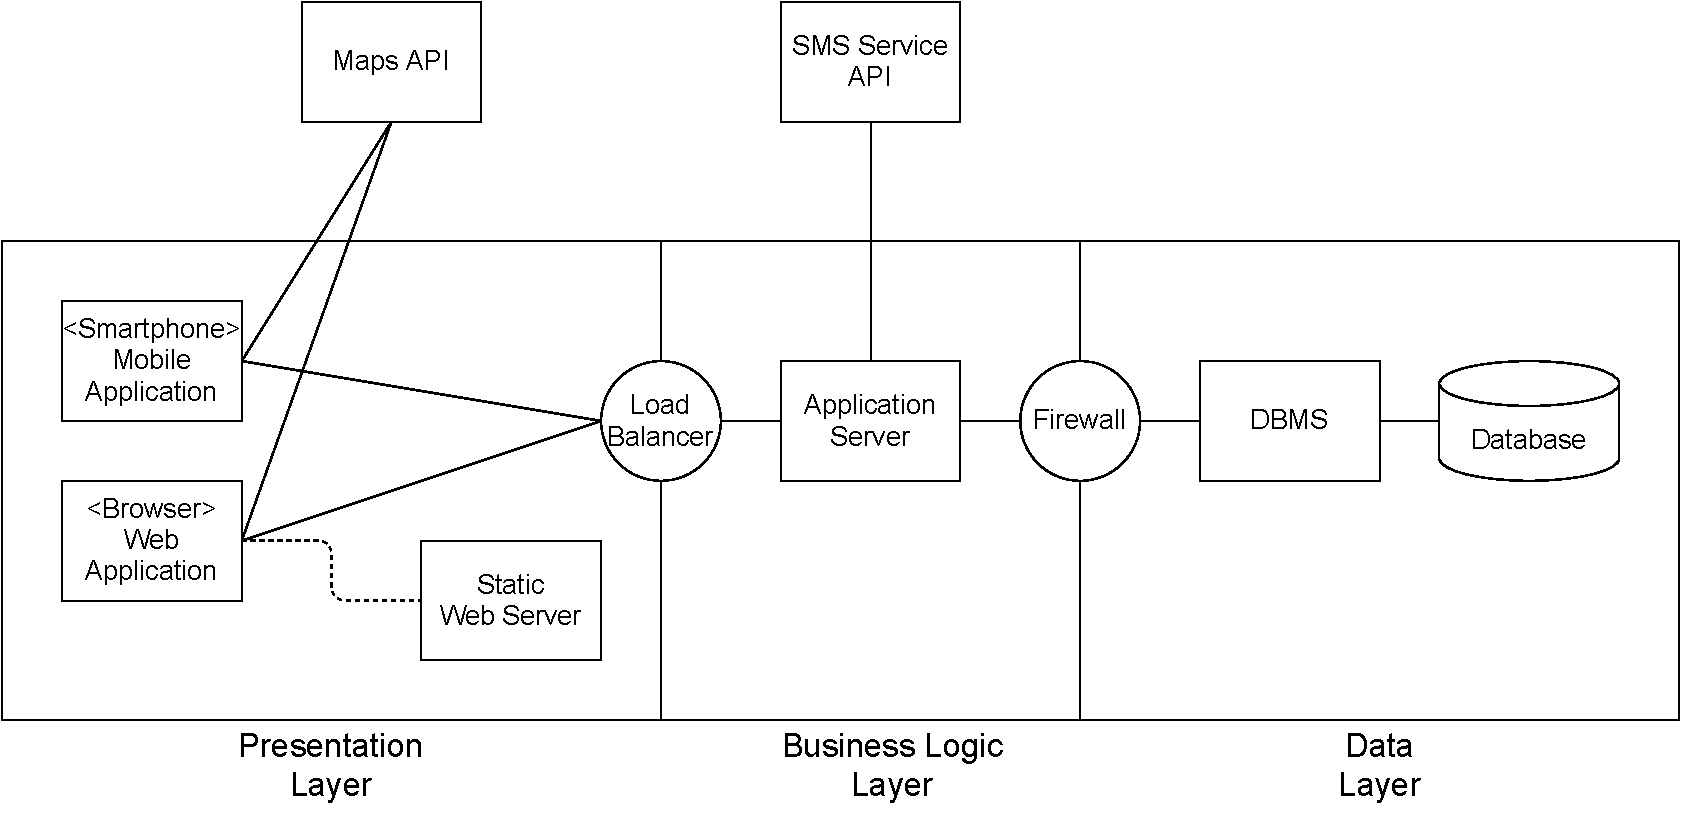
\includegraphics[width=\linewidth]{images/draw.io/overview_architecture.pdf}
    \caption{Overall architecture of the System}
    \label{fig:overview-architecture}
\end{figure}

The main components are the following:

\begin{itemize}
    \item \textbf{Mobile Application} The application is installed on the user's device through its store platform service. The application allows the user to interact with the service and receive notifications from the server.
    \item \textbf{Web Application} The web application allows users to access the same services available on the mobile app through any device, but it's not guaranteed that it can receive notifications. In addition to that, store managers may access a dedicated panel to configure additional parameters.
    \item \textbf{Static Web Server} It serves the client's browser a bundle that contains the web application code (compressed HTML and JS). It has no ties with the application server.
    \item \textbf{Application Server} It's the main backend component of the service, and contains the logic to process requests made against its API from the clients.
    \item \textbf{Database} It's the component that manages the connection to the database.
    \item \textbf{External Services} These services provides functionalities that the service can't provide by itself without additional infrastructure. They incluse a \emph{SMS Service} to send messages to users, a \emph{Notification Service} to send \emph{push} notifications to users and a \emph{Maps API} to visualize the location of the store on the user's device.
\end{itemize}

\subsection{Component View}
\begin{figure}[H]
    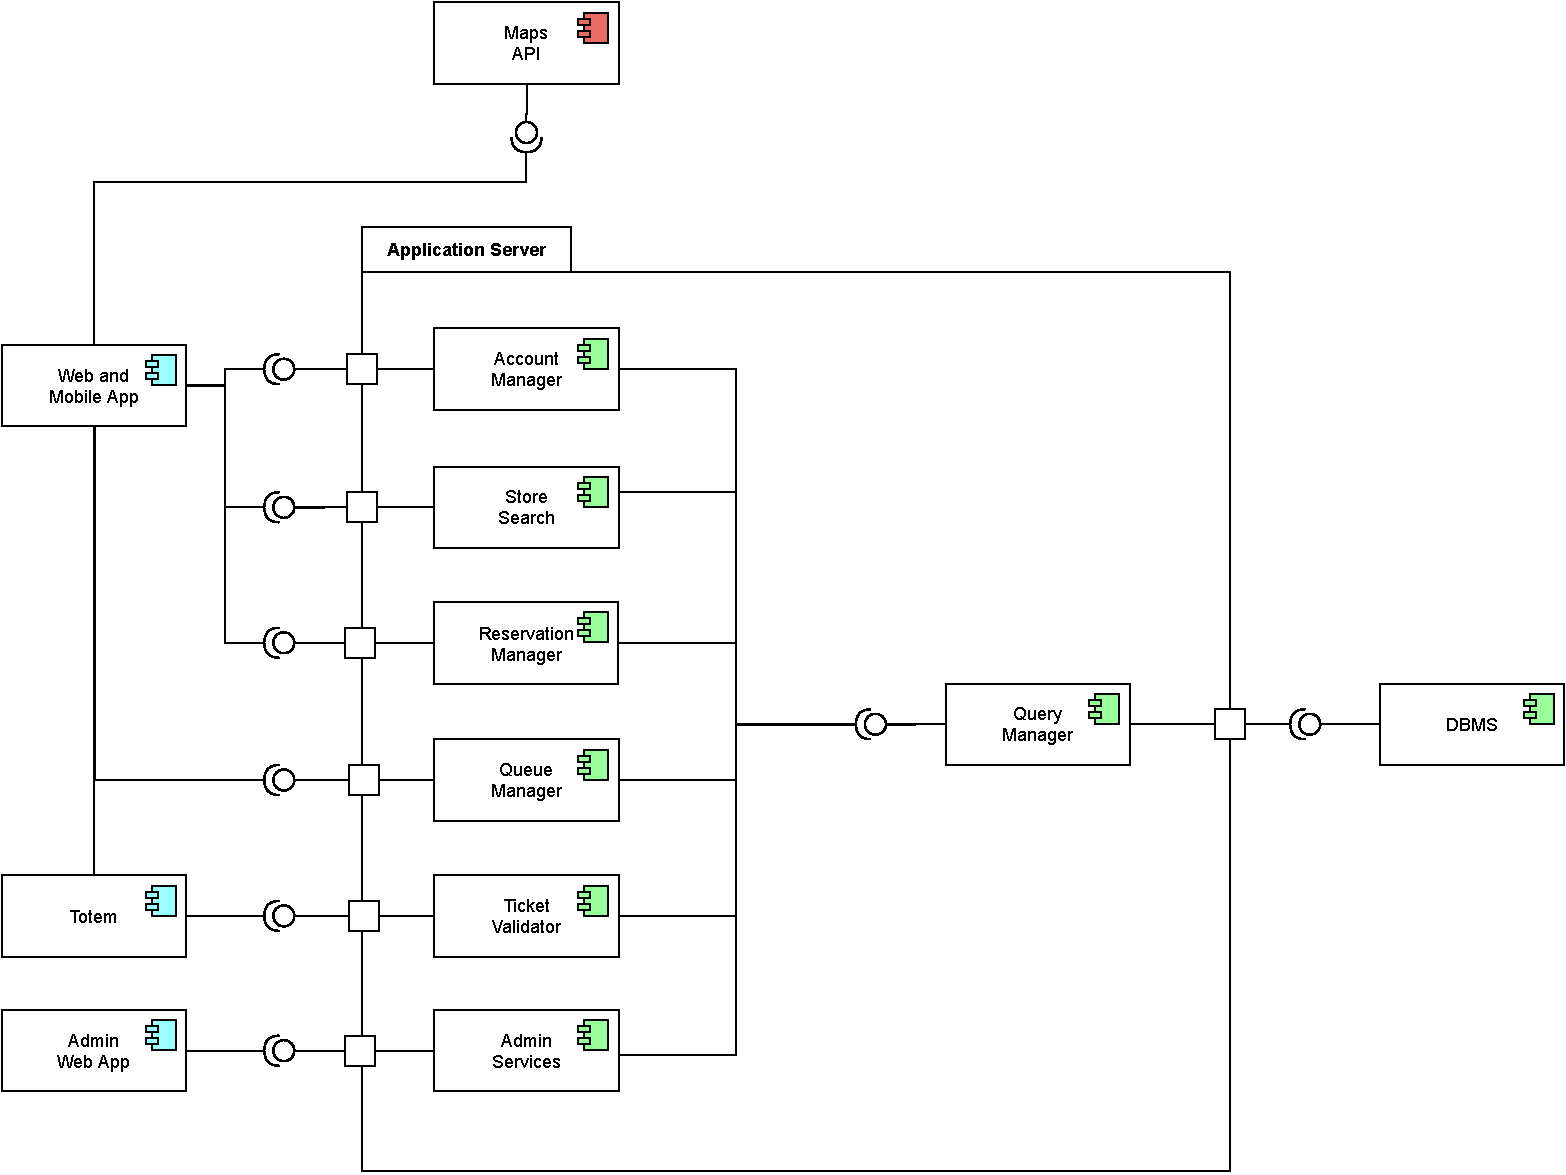
\includegraphics[width=\linewidth]{images/draw.io/component.pdf}
    \caption{Global Component Diagram of the System}
    \label{fig:component}
\end{figure}

\subsubsection{Data Base Structure}
The Data layer is composed of a relational database, and its associated DBMS will have the duty of processing and executing parallel requests.

Users and Admins will be stored in different tables.
Users can set up Free Timeslots Notifications, in order to be notified when a Timeslot at a specific day in a specific time range is made available for one of the favorite stores.
Users have an association with their Tickets, which include both Queue Tickets and Reservation Tickets.
In order to preserve the history of Users and for making data analytics possible, Tickets are never deleted, but instead are associated with a status indicating if they are currently active or already used.
Each Admin manages a number of Stores, having the power of changing their capacity or all details about their associated Timeslots.
Timeslots refer to a specific weekday and have an associated time.
In order to keep consistency with Reservation Tickets, Timeslots are immutable and never modified. Their status is instead set to inactive, and another Timeslot is created whenever a change has to be made.


\begin{figure}[H]
    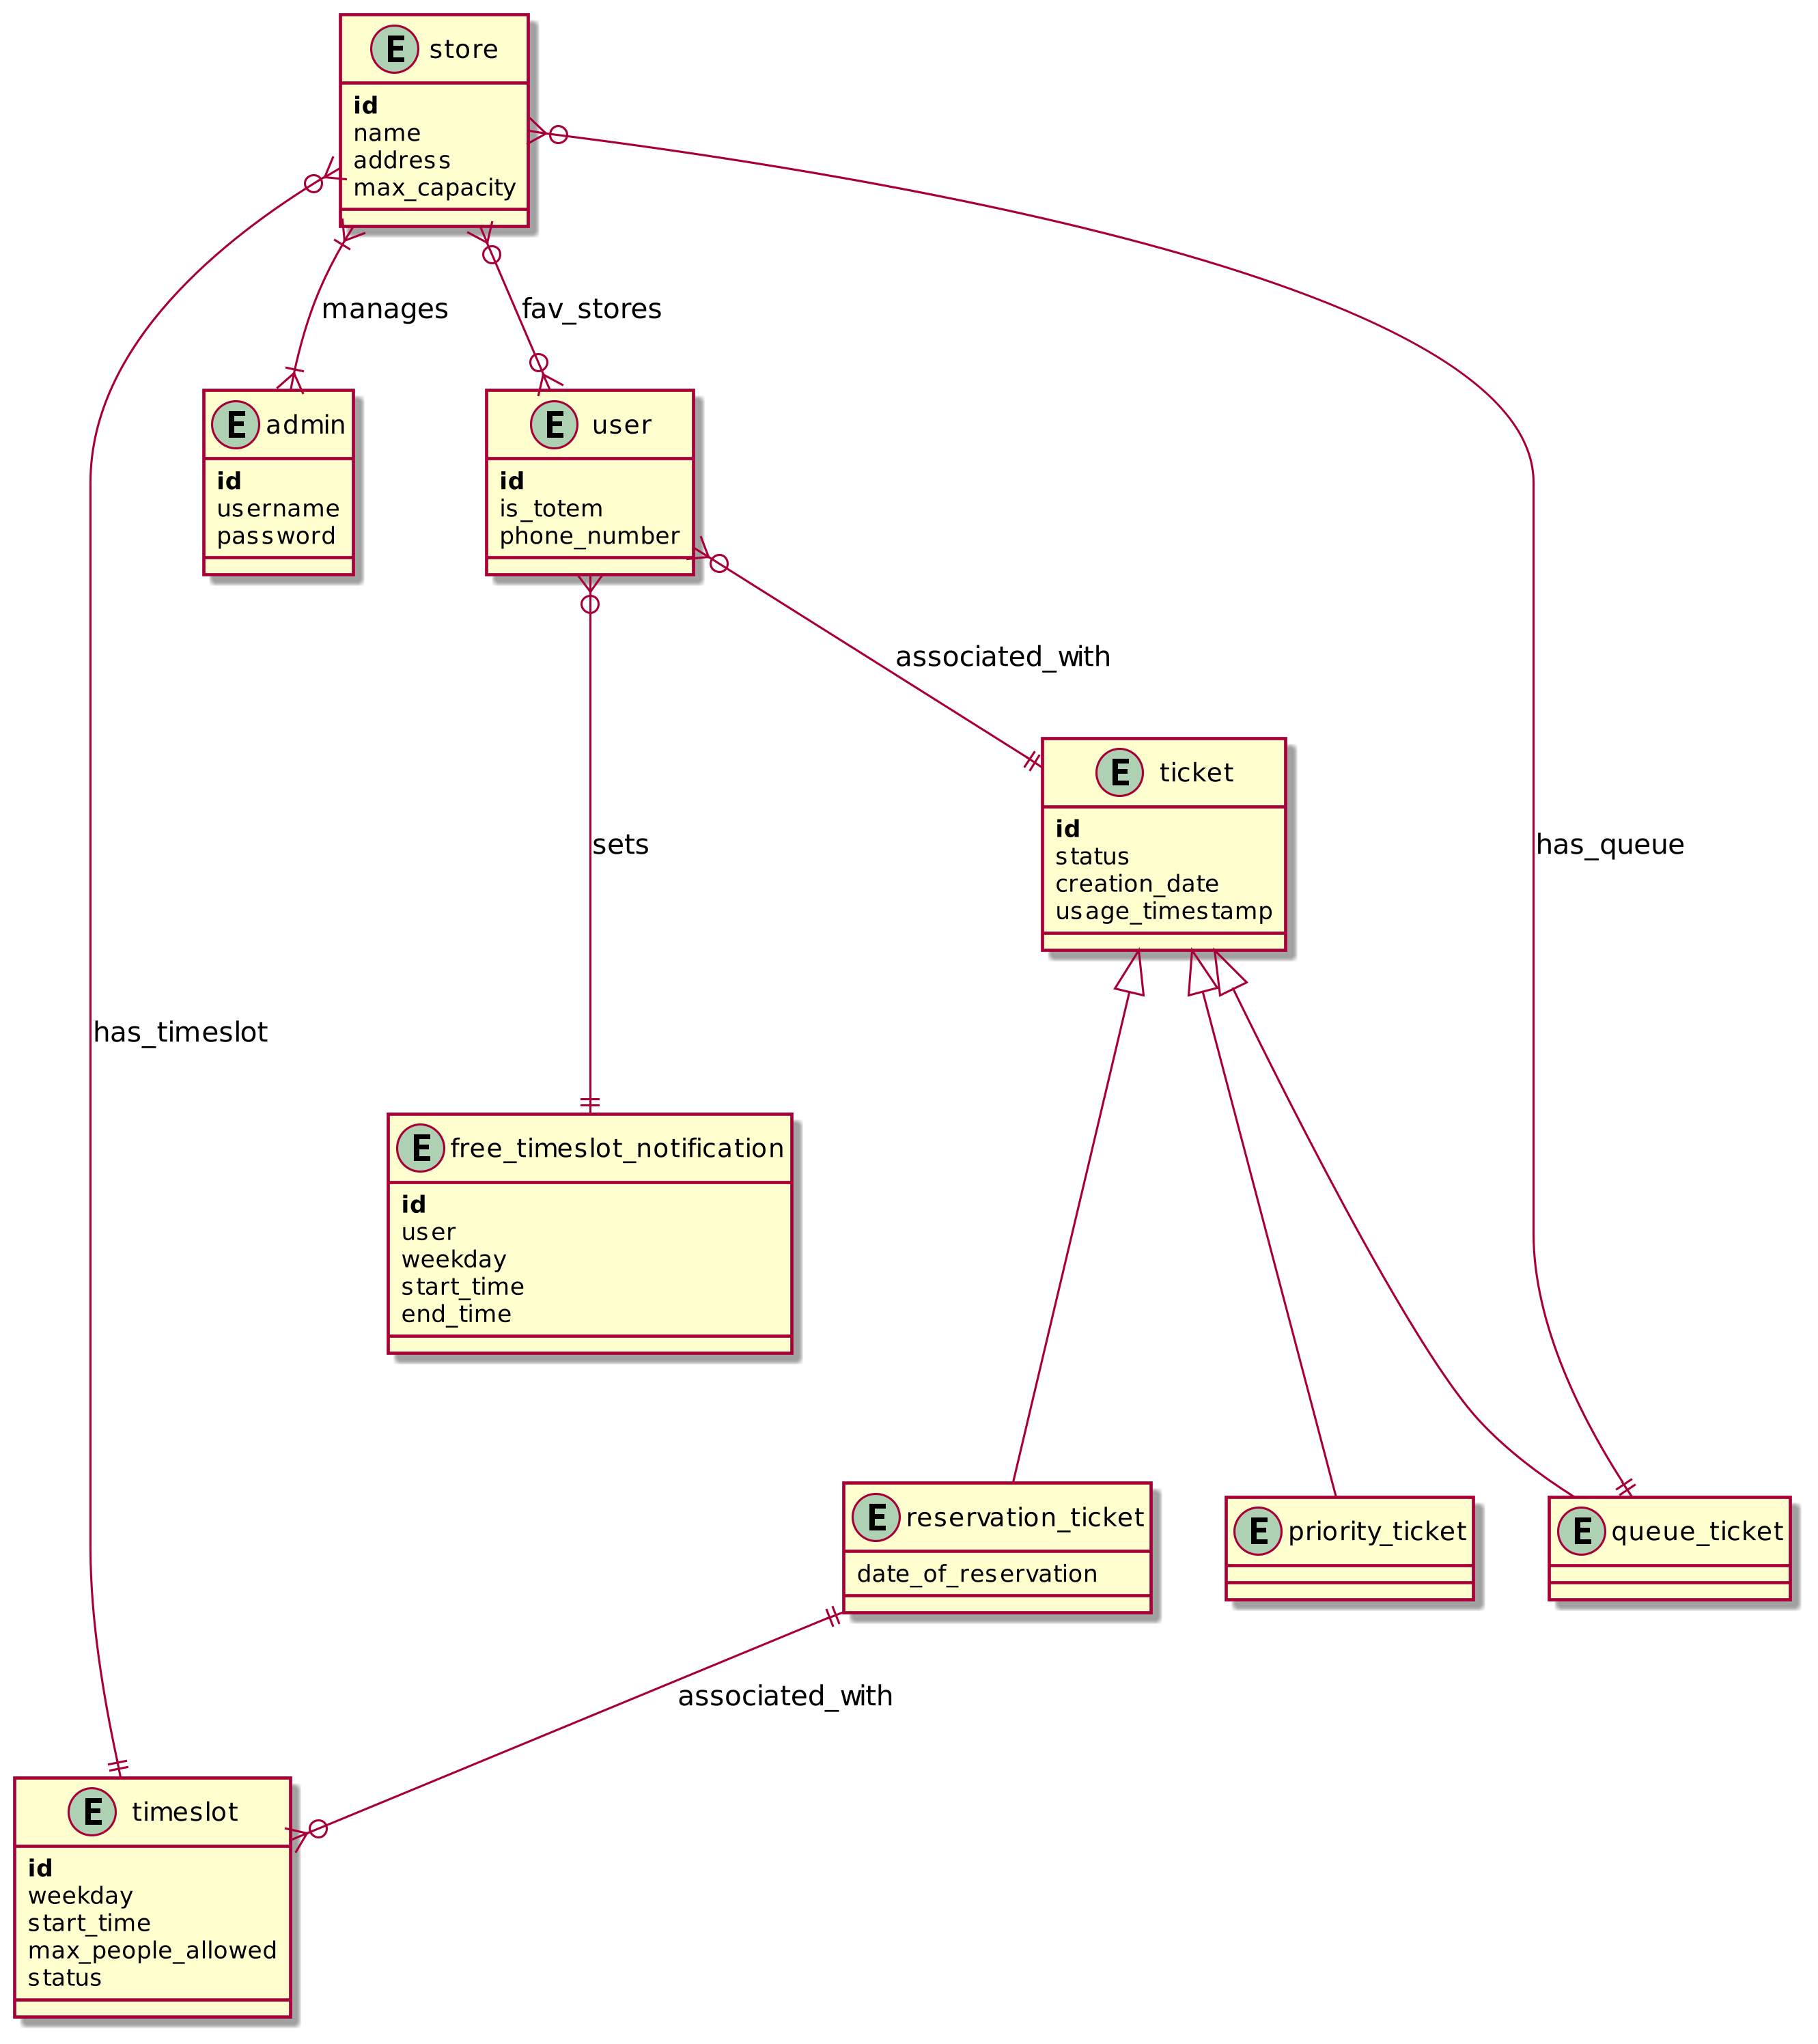
\includegraphics[width=\linewidth]{uml/db_structure.png}
    \caption{Data Base main structure}
    \label{fig:db_structure}
\end{figure}




\subsection{Deployment View}
Our system is composed of two independent components: a completely static webserver will be the access point where the client devices will fetch the one-page application, while the application server will offer the APIs to make it work.
For this reason we decided to use two different solutions.

The static webserver will make use of Cloudflare's content delivery network, in order to guarantee immediate response thanks to its edge location caches and reverse proxies.

The application server, composed of a business logic and a data tier, will be hosted on Amazon Web Services, making for easy scalability, replication, and load balancing.

\begin{figure}[H]
    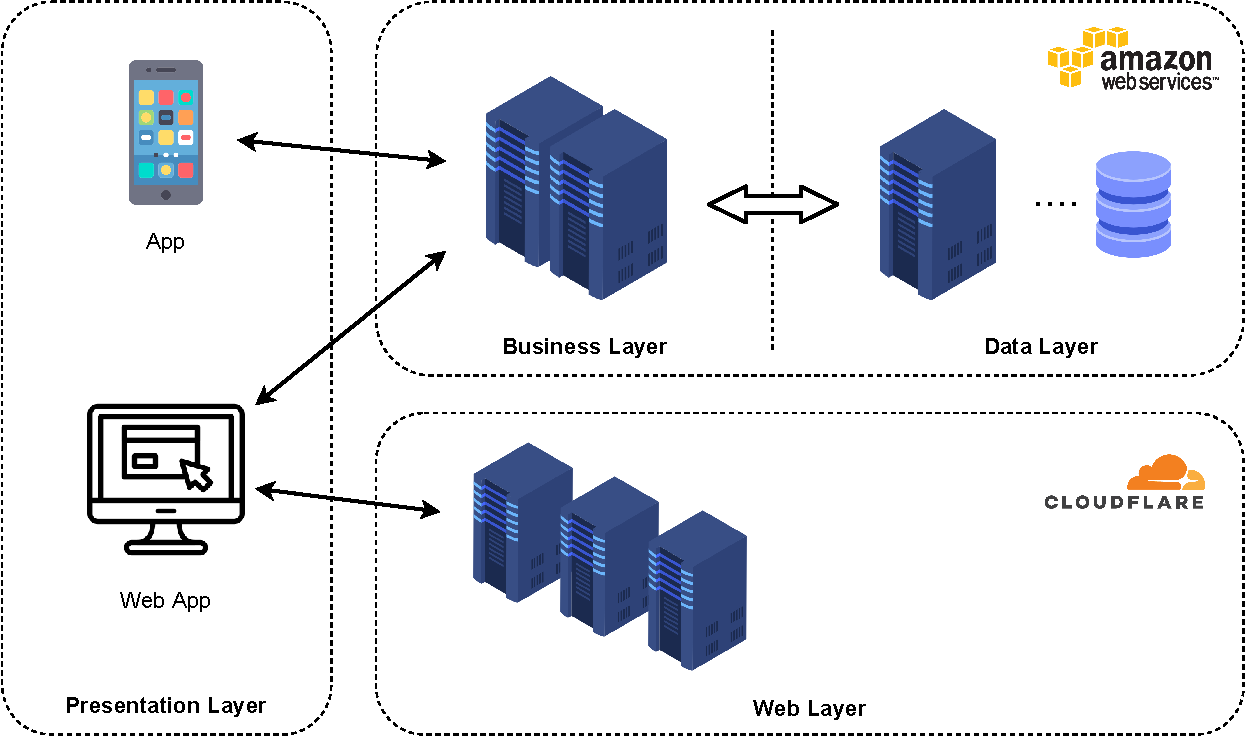
\includegraphics[width=\linewidth]{images/draw.io/deployment.pdf}
    \caption{Deployment View}
    \label{fig:deployment_view}
\end{figure}

\begin{figure}[H]
    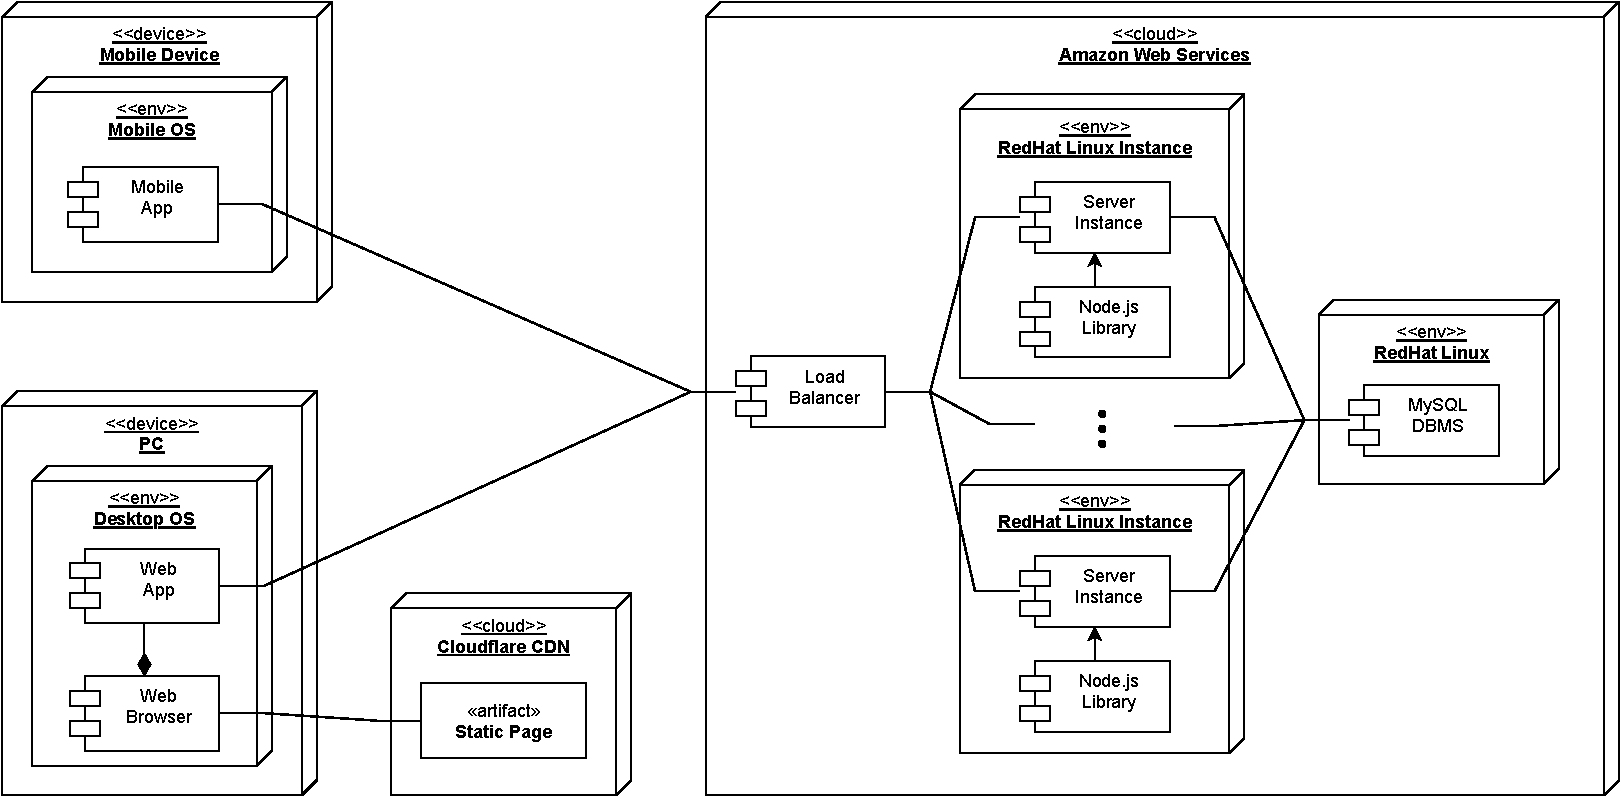
\includegraphics[width=\linewidth]{images/draw.io/deployment_structure.pdf}
    \caption{Deployment Structure}
    \label{fig:deployment_structure}
\end{figure}

\subsection{Runtime View}
% You can use sequence diagrams to describe the way components interact
% to accomplish specific tasks typically related to your use cases

\begin{figure}[H]
    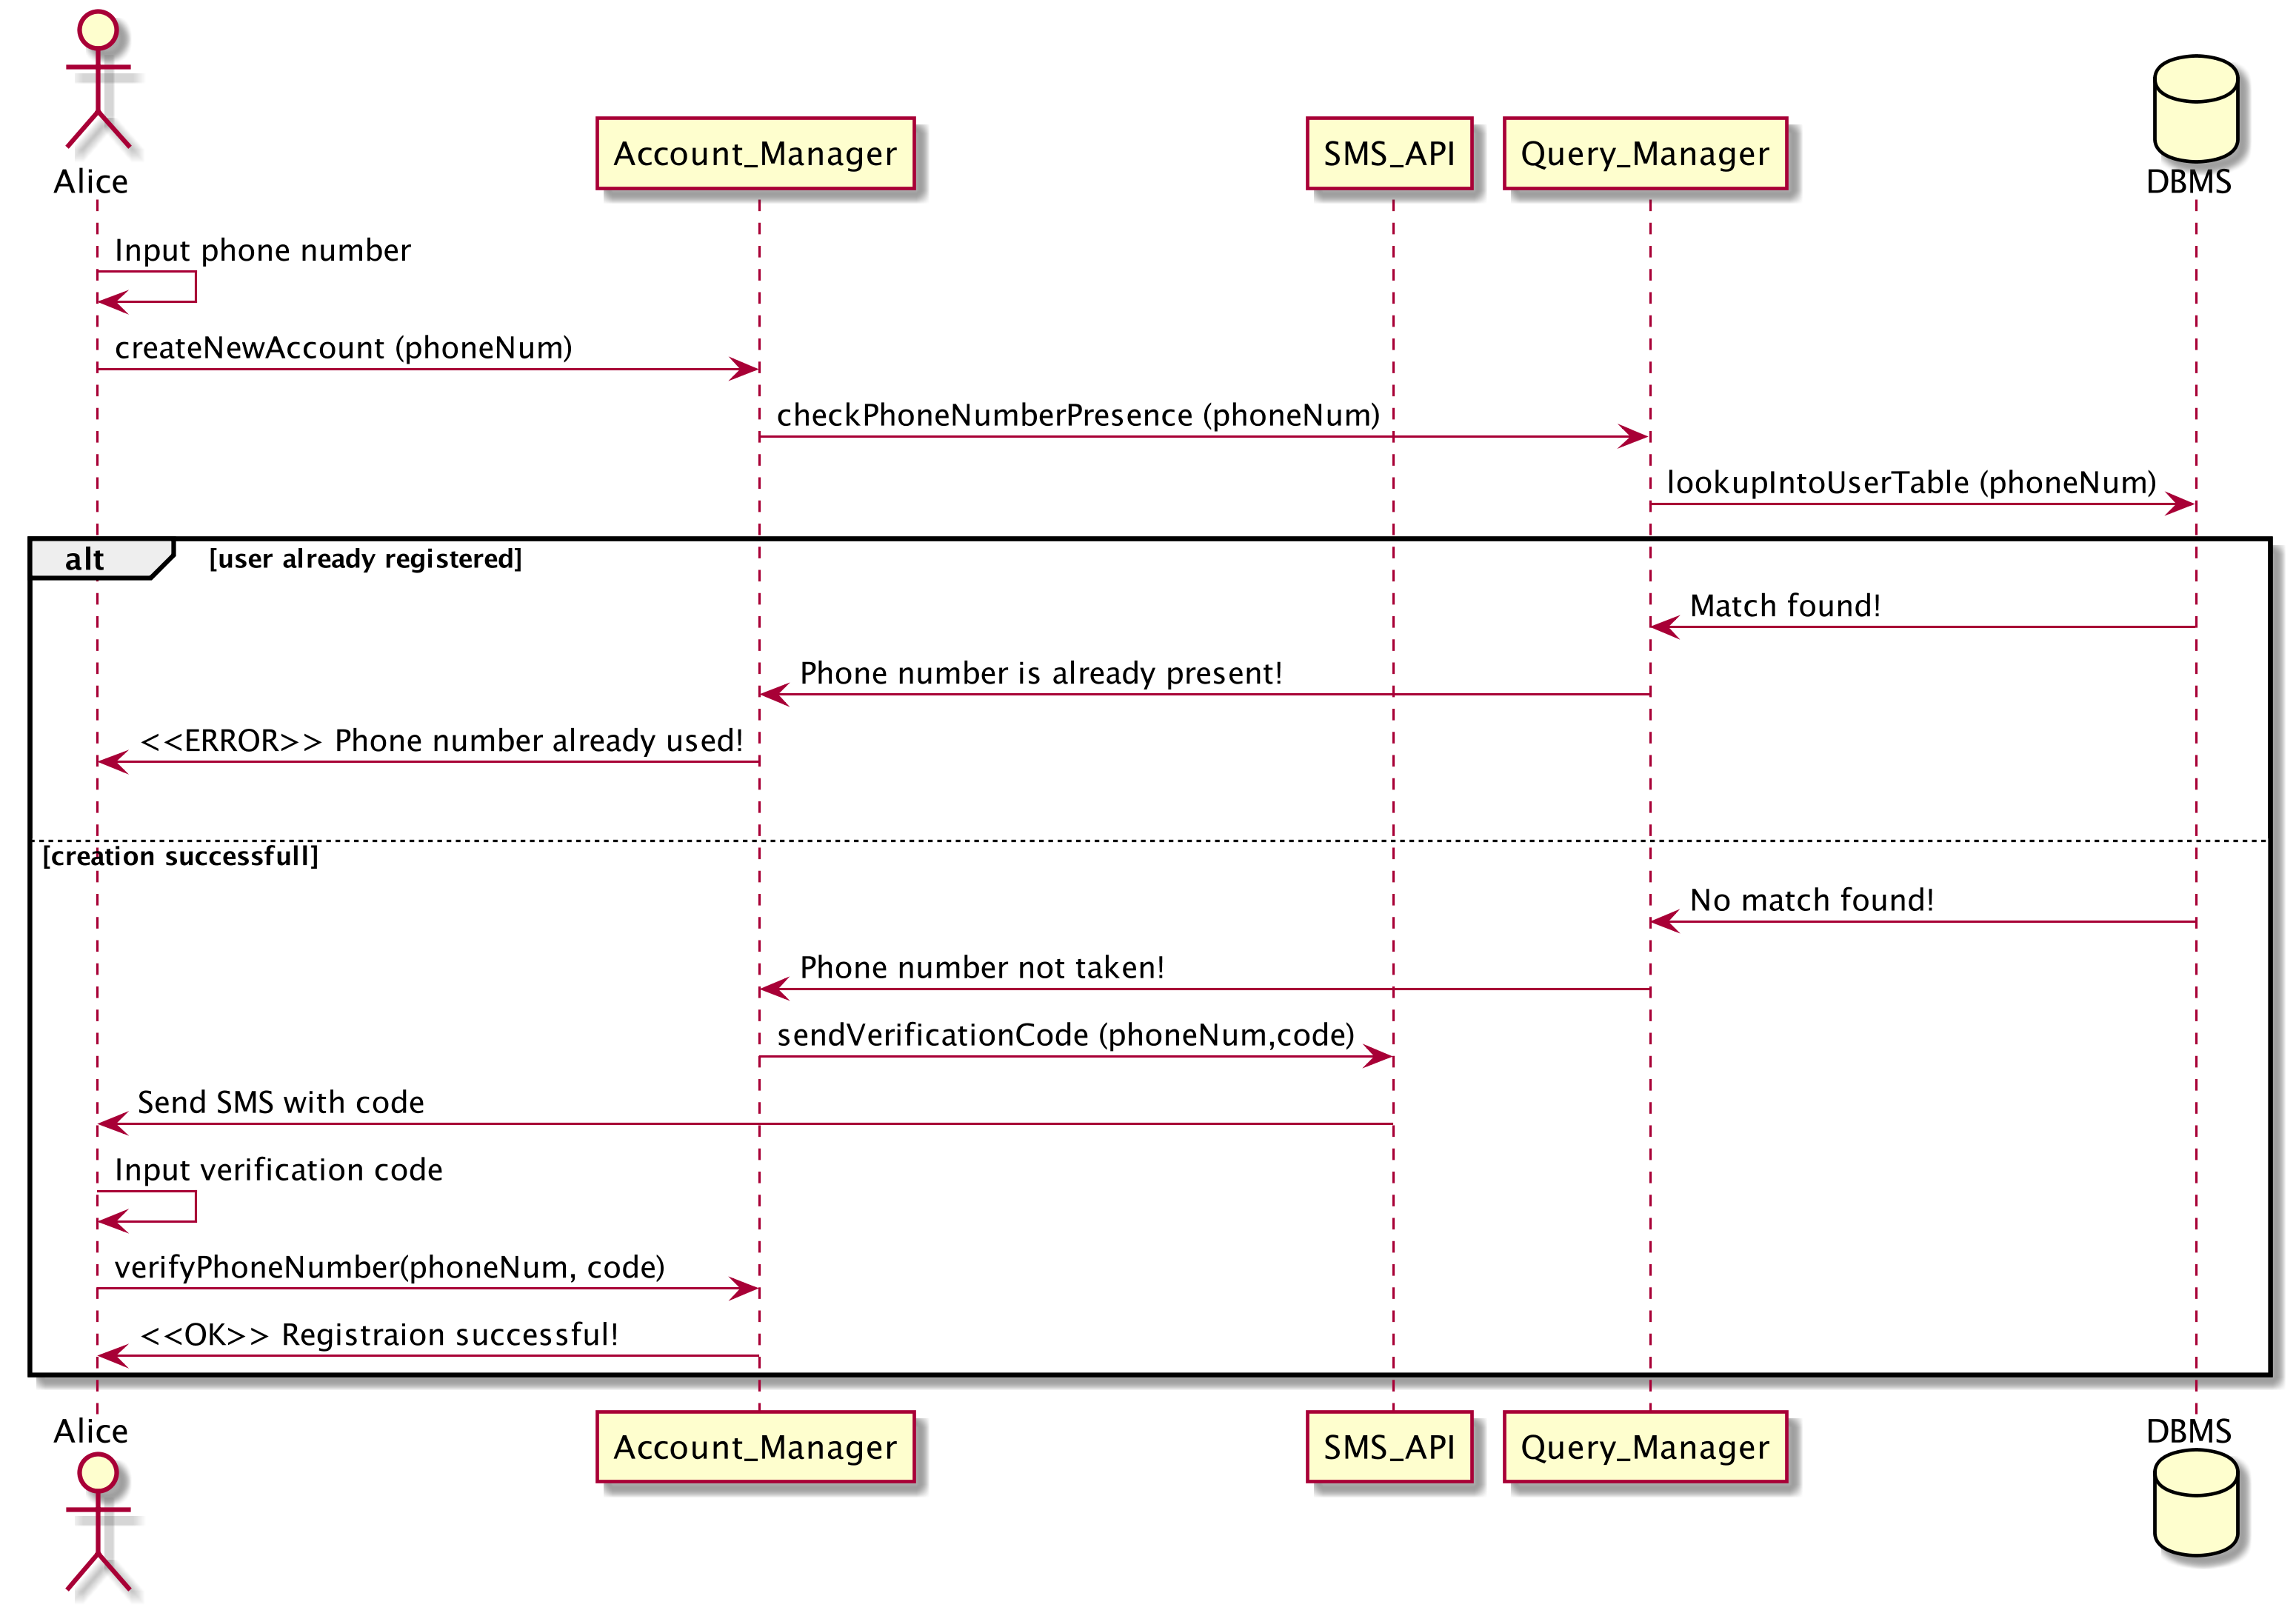
\includegraphics[width=\linewidth]{uml/seq_register_new_account.png}
    \caption{Register new account}
    \label{fig:seq_new_account}
\end{figure}




\subsection{Component Interfaces}

\subsection{Selected Architectural Styles and Patterns}
%  Please explain which styles/patterns you used, why and how
\subsubsection{Architectural Styles}
\paragraph{Thick Client}
The main characteristic of thick clients is offering a wide variety of functionalities independent from the central server.
The main advantages it offers are greater decoupling of frontend and backend and a reduced computational effort on the application server.
Recent years have seen a rise in the adoption of single page application, with the advent of rich framework which allow to write code that can be run both in an app and in the browser.
This allows developers to reuse great part of code across a large number of devices, all using the same API offered by the backend.
The one page application will be served by a dedicated static webserver, which logically separate from the rest of the system.

\paragraph{REST API}
REST is an architectural style centered around the definition of a uniform and predefined set of stateless operations defined on top of the HTTP protocol.
Its main advantages are simplicity, scalability and modifiability.

\paragraph{Three layer architecture}
Separating presentation, business, and data layers offers great flexibility, maintainability and scalability.
This combined with a thick client means that the only communication between the client and the server goes trough a predefined API, without having to worry about eachother's internal representation.

\subsubsection{Patterns}

\subsection{Other Design Decisions}
